% Distributed under the MIT License.
% (See accompanying file LICENSE.txt)
% (C) Copyright NoWork team

\documentclass[12pt,a4paper]{article}

\usepackage[utf8]{inputenc}
\usepackage[french]{babel}
\usepackage[T1]{fontenc}
\usepackage{verbatim}
\usepackage{graphicx}
\usepackage{listings}
\usepackage{hyperref}
\usepackage{lmodern}
\usepackage{listings}
\usepackage{textcomp} 
\usepackage{hyperref}
\usepackage{verbatim}

\title{NoWork\\
Analyse du cahier des charges}
\author{Équipe de développement NoWork\\[2em]}
\date\today

\newcommand{\latex}{\LaTeX\space}

\begin{document}
\maketitle

\section{Introduction}

Ce document analyse le cahier des charges initialement décrit par M. Frédéric Peschanski qui nous a été remis le 6 novembre 2013. L'objectif de ce travail est d'étudier les systèmes de réécriture afin de développer un logiciel permettant la réécriture de terme suivant une stratégie.

\section{Infrastructure technique}

\subsection{Dépendances}

\begin{itemize}
\item Compilateur OCaml 4.00.1 et la librairie standard OCaml ;
\item Le moteur de production \textit{GNU make} ;
\item Le moteur de production et de test \textit{ocp-build} version 1.99 ;
\item Le gestionnaire de paquet \textit{opam} version 1.1.0 ;
\item Le gestionnaire de version git.
\end{itemize}
\vspace{10pt}

Il n'y a pas de version web disponible donc il n'y a pas de dépendance vers \textit{js-of-ocaml}.

\subsection{Guide de style}

Le guide de style a été développé avec le client et est disponible en \latex dans le répertoire \verb=doc/coding-style.tex=. La documentation a été rédigée en \textit{OCamlDoc} et est disponible dans le répertoire \verb=doc/reference/=.

\subsection{Tests}

Le code est testé et les tests fonctionnels sont directement embarqués dans le langage. Les utilisateurs pourront donc eux-mêmes tester le code qu'ils auront écrit. Le répertoire \verb=data/test/= contient tous nos fichiers de tests et se décline en deux sous-dossiers \verb=run-fail/= et \verb=run-pass=, le premier contenant les fichiers testant les erreurs devant être déclenchées, et le deuxième testant qu'aucune erreur n'est lancée. Les tests unitaires sont réalisés dans le dossier \verb=tests/= et \textit{ocp-build} est utilisé pour déclencher ces tests.

\subsection{Organisation du projet}

Le cahier des charges initial spécifiait un module différent pour la représentation des termes et du système or il s'est avéré que les deux étaient trop fortement couplé et que des simplifications au niveau du code impliquait ses deux modules d'être unifié. Pour rappel, les modules sont :
\newline

\begin{itemize}
\item Module d'analyse lexicale et syntaxique (\verb=src/parser/=) ;
\item Module de représentation du système de réécriture et des termes (\verb=src/system/=) ;
\item Module de gestion du simulateur (\verb=src/algorithm=) ;
\item Module pour le \textit{top-level} (\verb=src/interactive=) ;
\item Module pour les tests unitaires (\verb=tests/=).
\end{itemize}
\vspace{10pt}

Il n'y a pas de module de gestion de l'exploration car cette fonctionnalité n'a pas été implémentée.

\section{Aspects algorithmiques}

Une partie du résultat attendu comporte une partie de recherche pour implémenter des structures de données et algorithmes en concordance avec les critères du client. Les prochaines sections donnent une idée du travail réalisé mais ne rentre pas dans les détails, pour les spécifications exactes, vous pourrez vous référer au document \verb=doc/pdf/dev-manual.pdf=.

\subsection{Structure de données}

Les termes sont représentés par un DAG avec partage maximal des sous-termes (via une structure de type \textit{hash-consing}). Les termes sont également représentés tel que l'opération d'égalité est complètement indépendante du nommage des termes, il y a une alpha-conversion implicite.
\newline
Le système de réécriture est représenté par une structure comprenant 4 environnements pour les \textit{kind}, les constantes, les opérations et les règles de réécriture.
\newline
La représentation des structures est complètement implémenté.

\subsection{Pattern matching nominal}

L'algorithme de pattern matching non-linéaire est implémenté grâce à la structure de \textit{hash-consing} citée précédemment et respecte donc la contrainte d'alpha-conversion.

\subsection{Réécriture nominale}

L'algorithme de réécriture nominale avec stratégie est complètement implémenté. Il est capable de réécrire des termes via des règles complexes comme celle du lambda calcul ou du langage concurrent CCS. Les différentes stratégies axiomatiques implémentées permettent de définir, à notre connaissance, n'importe quelle stratégie de plus haut niveau.

\subsection{Mode d'exploration}

Le mode d'exploration n'est pas complètement implémenté. L'algorithme de réécriture retourne un ensemble de termes et les prédicats ensemblistes d'égalité et d'inclusion sont implémentés. L'équivalence entre deux termes n'est pas implémentée mais le code existant permettrait de faire cette modification aisément car les préparatifs (tel que l'ensemble de termes) sont implémentés.

\section{Langage}

Cette partie n'était pas décrite dans le cahier des charges initial et a été ajoutée durant le projet.
\newline

La description et la vérification de la sémantique du langage est complètement implémentée. Nous pouvons distinguer 4 langages différents dans ce projet :
\newline

\begin{itemize}
\item Langage de description du système de réécriture avec typage comprenant les \textit{kind}, constantes, opérations et règles. Notons que les règles se décrivent avec deux sous-langages pour exprimer des \textit{patterns} et des \textit{effects}.
\item Langage de termes avec vérification des types, assez proche du langage de description des patterns.
\item Langage de stratégies comprenant les axiomes permettant de définir des stratégies de simulation.
\item Langage de commandes interactives permettant de faire des tests dans un \textit{top-level}.
\end{itemize}
\vspace{10pt}

\section{Aspects méthodologiques}

Le document \verb=doc/pdf/methodology.pdf= décrit en détail la méthodologie appliquée tout au long du projet. Rétrospectivement, plusieurs réunion, à raison d'une par mois environ, on été organisée avec le client en comité de 3 à 4 personnes.

La traçabilité du projet est garantie par l'utilisation de \textit{rallydev} qui nous a permis d'appliquer la méthode Scrum. Les itérations duraient entre 2 à 3 semaines et des pauses dans le développement ont été organisée pendant les examens qui pouvait s'étaler sur 3 semaines parfois.

\section{Livrable}

Le livrable est constitué :
\newline

\begin{itemize}
\item Du code source dont tous les .mli sont correctement documentés.
\item D'un jeu de scénarios utilisateurs qui suivent dans ce document.
\item D'un guide utilisateur (\verb=doc/user-manual.tex=)
\item D'un guide développeur (\verb=doc/dev-manual.tex=)
\end{itemize}
\vspace{10pt}

Le tous sera livré via une \textit{pull-request} dans le dépôt officiel Github (\url{https://github.com/fredokun/nominal-workbench}).


\section{Cas d'utilisation}

La liste des fonctionnalités interactives est montrée dans le diagramme de cas
d'utilisation à la figure~\ref{use-cases}. La suite présente plus en détails les différents cas d'utilisation.

\begin{figure}[h!]
  \centering
  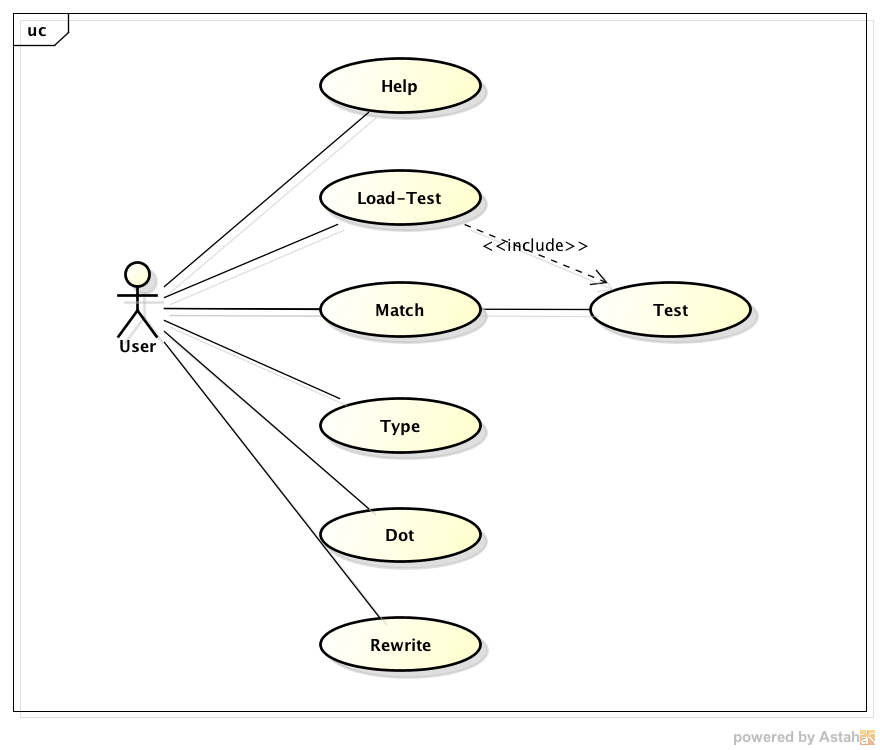
\includegraphics[width=\linewidth,natwidth=\linewidth,natheight=\textheight]{use-case-diagram.png}
  \caption{List of use cases for nowork}
  \label{use-cases}
\end{figure}

\begin{description}

\item[Help:]
Affiche la liste des commandes disponibles suivie de la description des options.

\begin{minipage}{\textwidth}
Résultat de la commande \verb=:help= :
\begin{lstlisting}[breaklines=true,basicstyle=\ttfamily\footnotesize]
Available commands :
        :help            -- Displays this help
        :?               -- Displays this help
        :load-test f exp -- Load a test file f and check that the result matches the expectation
        :test            -- Test an expression (consult user-doc for more infos)
        :match           -- Check that an expression matches the given type or strategy
        :type            -- Returns the type of the expression
        :dot t out       -- Output the hash-consed version of a term into a dot file graph
        :quit            -- Exits the REPL
        :exit            -- Exits the REPL
        :q               -- Exits the REPL
More detailled informations may be found in the user documentation
\end{lstlisting}
\end{minipage}

\item[Load-test:]
Permet de charger un fichier texte, de l'exécuter et de vérifier que le résultat est celui attendu. L'utilisateur peut s'assurer qu'un fichier est syntaxiquement correct et que les tests écrits dans ce fichier passent.

\begin{minipage}{\textwidth}
Exemple :
\begin{lstlisting}[breaklines=true,basicstyle=\ttfamily\footnotesize]
> :load-test "data/test/run-fail/typecheck_unification2.nw" --failwith RewritingSystemError.TypeClash ;;
    Filename: data/test/run-fail/typecheck_unification2.nw
    [ passed ]  Failure with RewritingSystemError.TypeClash as expected.
        Info: Type clash between A and K2.
\end{lstlisting}
\end{minipage}

\item[Test:]
Permet de tester que l'ensemble des termes renvoyé par une réécriture est égal ou inclus dans le deuxième argument du prédicat.\\

 \begin{minipage}{\textwidth}
Exemple :
\begin{lstlisting}[breaklines=true,basicstyle=\ttfamily\footnotesize]
> :test rewrite Add(Zero,Successor(Zero)) with Bottomup --equal Successor(Zero)
  Terms : Lambda (x, Var (x)) rewrote into :Lambda (x, Var (x))
[ passed ]  Terms have been correctly rewritten in : Lambda (x, Var (x));;
\end{lstlisting}
\end{minipage}

\item[Type:]
Permet d'obtenir le type d'un terme.\\

\begin{minipage}{\textwidth}
Exemple :
\begin{lstlisting}[basicstyle=\ttfamily\footnotesize]
> :type Lambda(x, Var(x));;
   Term
\end{lstlisting}
\end{minipage}

\item[Dot:]
Permet de générer un fichier dot avec la représentation \textit{hash-consé} d'un terme. \\

\begin{minipage}{\textwidth}
Exemple :
\begin{lstlisting}[basicstyle=\ttfamily\footnotesize]
> :dot Lambda(x, Var(x)) "lambda.dot" ;;
\end{lstlisting}
\end{minipage}

\item[Match:]
Permet de voir si une terme match un pattern donné. \\

\begin{minipage}{\textwidth}
Exemple :
\begin{lstlisting}[basicstyle=\ttfamily\footnotesize]
> :match App(Lambda(x, Var(x)), Lambda(y, Var(y))) 
       --with App(?T, ?T)
\end{lstlisting}
\end{minipage}

\item[Quit:]
Arrête le programme.

\end{description}

\end{document}

